\documentclass[../Main/main.tex]{subfiles}

\begin{document}
\graphicspath{{../Flow in porous media/figs/}}
\chapter{Flow in Porous Media}
In this chapter we introduce the basic concepts of flow in porous media, briefly covering the modeling choices and physics that leads to Richards' equation. The theory in this chapter is to a large extent adapted from \cite{Nordbotten} and UIB's Porous media course.
\section{The Representative Elementary Volume}\label{REV}
\addcontentsline{toc}{section}{The REV}
A porous medium consists of a solid matrix and some void filled with fluid of one or more phases. In porous media research, one has come to the realization that the solid matrix is too complex to model. Instead one takes averages of variables over a reasonable length scale, ie. the \emph{representative elementary volume} (REV).
An important characterization of a porous medium is the \emph{porosity} $\phi$, it is defined as 
\begin{equation}
	\phi := \frac{\textit{volume of voids in REV}}{\textit{volume of REV}}.
\end{equation}
Another measure is the \emph{saturation} $S_{\alpha}$ of phase $\alpha$,  this is defined 
\begin{equation}
	S_{\alpha} := \frac{\textit{volume of }\alpha \textit{ in REV}}{\textit{volume of voids in REV}}.
\end{equation}
In single phase flow, the saturation is irrelevant as the saturation is always one. Also note that the volumetric content of phase $\alpha$ in the REV, $\theta_{\alpha}$, is given by $\theta_{\alpha} = S_{\alpha} \phi$.

\section{Darcy's Law}
\addcontentsline{toc}{section}{Darcy's law}
In 1856, Henri Darcy performed a famous experiment where he studied the flow of water through sand. To understand his experiment we must first define some variables for measuring water content. First, we assume that the external gravitational force on some fluid is balanced by the pressure gradient force, also known as \emph{hydrostatic equilibrium}. Then the pressure at height $z$ above datum developed by a water column of height $h$ above datum is given by
\begin{equation*}
p_{abs}(z) = p_{atm} + \rho g(h-z).
\end{equation*}
Where $\rho$ is the density and $g$ is the standard gravitational acceleration.
If we define the \emph{gauge pressure} $p$ by $p := p_{abs}-p_{atm}$ we get an expression for $p$:
\begin{equation*}
p = \rho g(h-z).
\end{equation*}
This can be rearranged to give an expression for the height, which we from now on refer to as \emph{hydraulic head}:
\begin{equation}\label{eq:hydraulic}
h = \frac{p}{\rho g} + z.
\end{equation}
A \emph{manometer} is a tube with one end in the reservoir and one in open atmosphere, the water level in this tube is then $h$. The volumetric flow of water is denoted by $q_d$. Darcy's experiment is shown in figure \ref{fig:darcy}, where water is poured through a cylinder filled with sand. The cylinder has length $L$ and has cross sectional area $A$. His observations are given by the equation called Darcy's law:
\begin{equation}
q_d = -\kappa \frac{A(h_2-h_1)}{L}.
\end{equation}
Where $\kappa$ is a positive coefficient of proportionality.
\begin{figure}[h]
\centering
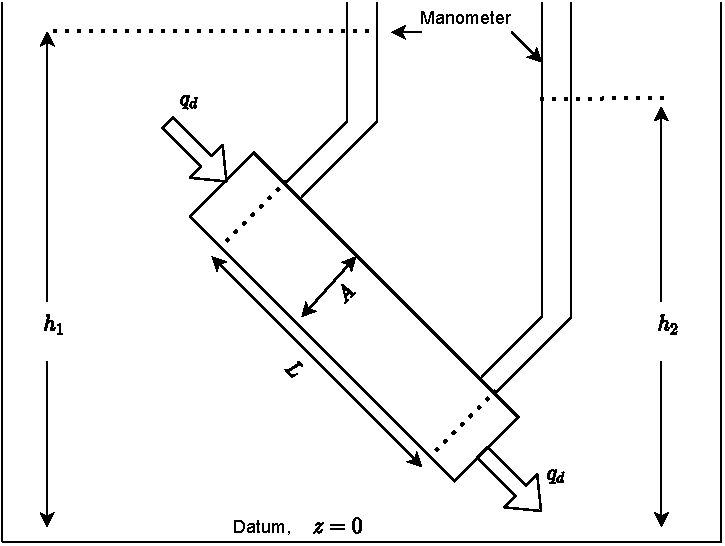
\includegraphics[width=0.9\textwidth]{Darcy experiment.pdf}
\caption{The Darcy experiment}
\label{fig:darcy}
\end{figure}Let $q$ denote the volumetric flow-rate per area:
\begin{equation*}
q := \frac{q_d}{A} = -\kappa \frac{h_2-h_1}{L},
\end{equation*}
we will refer to this as the \emph{flux} of hydraulic potential. We can now state the differential version of Darcy's law. Taking the limit as $L\rightarrow 0$ we get 
\begin{equation}\label{eq:darcy}
\bm{q} = -\bm{\kappa} \nabla h.
\end{equation}
We call $\bm{\kappa}$ the \emph{hydraulic conductivity} and note that it in general is a rank two tensor, a matrix. The \emph{hydraulic conductivity} also has the property that it is \emph{symmetric}: This is because there are, at every point in the reservoir, two orthogonal directions; one with maximum, and one with minimum hydraulic conductivity. Thus, the matrix, $\bm{\kappa}$, is diagonalizable by a orthogonal matrix.\par
The conductivity matrix, $\bm{\kappa}$, is also \emph{positive definite}, this is because there is never flux in the same direction as the pressure gradient. 
With further experiments, similar to the one already described, we can understand what makes up $\bm{\kappa}$. Dimensionality analysis shows that it is  a function of viscosity $\mu$, density of the fluid $\rho$, gravity $g$ and \emph{permeability} $\bm{k}$,
\begin{equation} \label{eq:conductivity}
\bm{\kappa} = \frac{\bm{k} \rho g}{\mu}.
\end{equation}
The \emph{permeability}, which is a property of the soil in the reservoir, is also a rank two tensor which is symmetric positive definite and is in general a function of space, ie. heterogeneous.
\par If we define the \emph{pressure head} $\psi$ as $\psi := \frac{p}{\rho g}$, we can combine \eqref{eq:hydraulic}, \eqref{eq:darcy} and \eqref{eq:conductivity} to get another variant of Darcy's law;
\begin{equation}\label{eq:darcyv2}
\bm{q} = -\frac{\bm{k}\rho g}{\mu}\nabla(\psi + z)
\end{equation}
 which will be useful later.
\section{Mass Conservation}
\addcontentsline{toc}{section}{Governing equations}
Darcy's law is not enough if we want to determine the pressure or flow in a reservoir, but we can use the principle of \emph{mass conservation} to add one more equation. 
The idea is that for every enclosed region in the reservoir, the change of mass inside the region is balanced by the mass flux into the region and the production of mass inside the region.
\\
We end up with the mass balance equation, let $\Omega$ be our domain, then:
\begin{equation*}
\int_{\omega}\frac{\partial (\rho \phi) }{\partial t} dV= -\int_{\partial\omega}\bm{n}\cdot\rho\bm{q} \ dS+\int_{\omega} f dV \ \ \forall \omega \subseteq \Omega \ \ \text{with }\omega \text{ being a volume,}
\end{equation*}
where $\bm{n}$ is an outward pointing normal vector to $\omega$ and $f$ corresponds to sources and/or a sinks. We can use the divergence theorem on the surface integral to get
\begin{equation*}
\int_{\omega}\frac{\partial (\rho \phi) }{\partial t} + \nabla \cdot(\rho \bm{q}) -fdV= 0.
\end{equation*}
Since this is true for all enclosed regions $\omega\subset \Omega$, it also holds for the expressions inside the integral yielding the mass conservation PDE
\begin{equation*}
\frac{\partial (\rho \phi) }{\partial t} + \nabla \cdot (\rho \bm{q}) = f.
\end{equation*}
This, together with Darcy's law \eqref{eq:darcy} and appropriate boundary and initial conditions close the system
\begin{equation}\label{eq:singlephase}
\left \{ \begin{aligned}
	\bm{q} &=-\bm{\kappa} \nabla h, & \bm{x} &\in \Omega,  &t &>0 \\
	\frac{\partial (\rho \phi) }{\partial t} + \nabla \cdot(\rho \bm{q}) &=f(\bm{x},t), & \bm{x} &\in \Omega, & t &>0 \\
	h(\bm{x}) &= g(\bm{x},t), &\bm{x} &\in \partial \Omega,&t &>0 \\
	h(\bm{x}) &= f(\bm{x}), & 	\bm{x} &\in \Omega,  &	t &=0 
\end{aligned}\right. 
\end{equation}
Now we have a model for single-phase flow. As it is stated now, it is a linear parabolic equation, but for incompressible fluid and matrix it becomes an elliptic equation. One often writes the density as a function of pressure, it then becomes non-linear. See chapter two of \cite{Nordbotten} for a more detailed discussion of \eqref{eq:singlephase} and modelling options.

\section{Two-phase Flow and Richards' Equation}
\addcontentsline{toc}{section}{Twophase flow and Richards' equation}
We restrict our discussion to two phases for simplicity, but the theory can be extended to more phases. In two-phase systems one has a \emph{wetting phase} and a \emph{non-wetting phase}. Denoted by the subscripts $w$ and $n$, respectively. \\
When we introduce more phases, we continue with the equations we already introduced, ie. we assume that Darcy's law  \eqref{eq:darcyv2} holds for both phases. Let the subscript $\alpha$ denote the phase, then we have Darcy's law for each phase
\begin{equation}\label{eq:darcytwo}
	\bm{q}_{\alpha} = \frac{\bm{k}_{r,\alpha}\bm{k}\rho g}{\mu}\nabla(\psi_{\alpha} + z),
\end{equation}
where the coefficient $\bm{k}_{r,\alpha}$ is known as \emph{relative permeability} and it has to be deduced from experimental observation. \par We also assume conservation of mass for each phase:
\begin{equation}\label{eq:massbalancetwo}
	\frac{\partial (S_{\alpha}\rho_{\alpha} \phi) }{\partial t} + \nabla \cdot (\rho \bm{q}_{\alpha}) = f_{\alpha}.
\end{equation}
Here, we assume that there is no mass transfer between the phases.
If we combine equations \eqref{eq:darcytwo} and \eqref{eq:massbalancetwo}, they give us $2$ equations, but we have four unknowns $\psi_w$, $\psi_n$, $S_w$ and $S_n$. We, therefore, introduce the algebraic relation
\begin{equation*}
	S_w + S_n = 1
\end{equation*}
and the physical relation
\begin{equation}\label{eq:capillary pressure}
	p_n-p_w = p_c
\end{equation}
where $p_c$ is called \emph{capillary pressure}. As with the relative permeability, $p_c$ also need to be determined experimentally.
With initial and boundary conditions we again have a closed system.\par
A common simplification is to assume that the capillary pressure and the relative permeability are functions of the saturation, and that the relative permeability is isotropic (a scalar). \par
Another simplification that is used, especially in groundwater hydrology, is that the non-wetting phase (air) always have $p_n = p_{atm}=0$. For this assumption to hold it is important that the air always is connected to the surface. Now, equation \eqref{eq:capillary pressure} simplifies to
\begin{equation*}\label{eq:groundwater capillary pressure}
	-p_w = -\psi_w\rho g = p_c(S_w).
\end{equation*}
Experiments show that the capillary pressure is a monotone decreasing function of saturation, therefore we can invert it. Equation \eqref{eq:capillary pressure} now becomes:
\begin{equation*}
	P_c^{-1}(\psi_w\rho g) = S_w.
\end{equation*}

Finally, we can multiply the above equation by the porosity to get an expression for the \emph{water content} $\theta_w$:
\begin{equation*}
	\theta_w = \theta_w(\psi_w) = \phi P_c^{-1}(\psi_w\rho g).
\end{equation*}  
Combining this with the two-phase Darcy law \eqref{eq:darcytwo} and mass balance \eqref{eq:massbalancetwo} we get \textbf{Richards' equation}
\begin{equation}\label{eq:richards}
	\frac{\partial \theta(\psi)}{\partial t} - \nabla \cdot (\bm{\kappa} (\theta (\psi))(\nabla \psi + e_z)) = f
\end{equation}
where $\theta = \theta_w$. Note that the density is eliminated, this is because it is assumed to be constant for water. The hydraulic conductivity is parametrized as a function of water content through experiments and can be written  $\frac{\bm{k}_{r,\alpha}\bm{k}\rho g}{\mu} = \bm{\kappa}(\theta)$. \par 
Richards' equation contains two non-linearities, $\theta$ and $\bm{\kappa}$, which make the analysis and numerical simulation more interesting and challenging as we will see. They may also cause the equation to degenerate, ie. the parabolic equation may "collapse" into an elliptic PDE (see figure \ref{fig:richards} ) or even an ODE.
\begin{figure}[h]
	\centering
	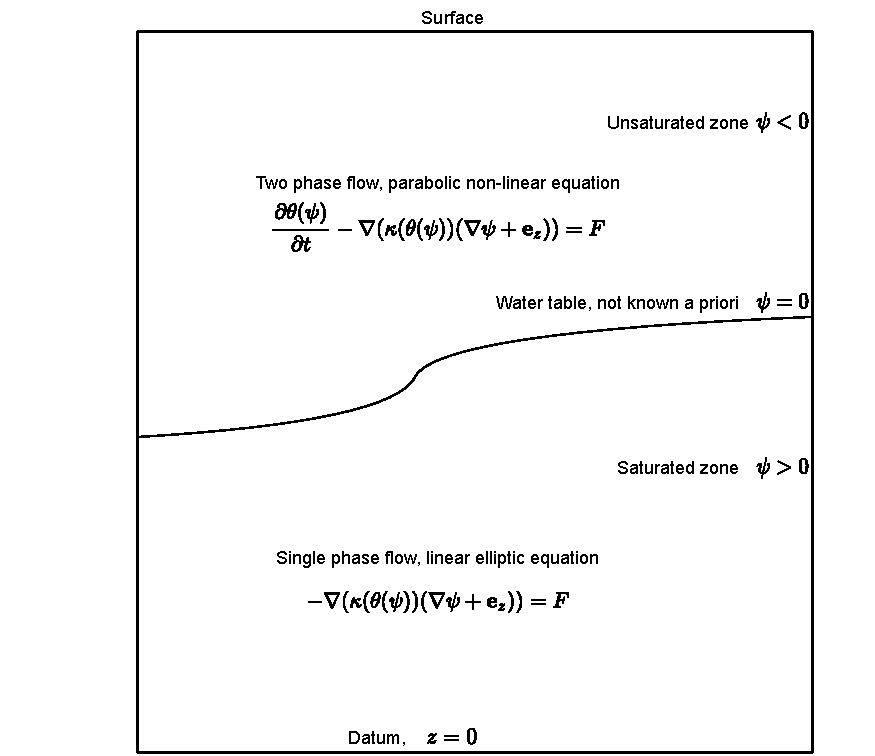
\includegraphics[width=\textwidth]{Richards.pdf}
	\caption{A sketch of the degeneracy of Richards' equation}
	\label{fig:richards}
\end{figure}
 \end{document}